\documentclass{article}
\usepackage{enumerate}
\usepackage{amsmath}
\usepackage{amssymb}
\usepackage{graphicx}
\usepackage{subfigure}
\usepackage{geometry}
\geometry{left=3.0cm,right=3.0cm,top=3.0cm,bottom=4.0cm}
\renewcommand{\thesection}{Problem \arabic{section}.}

\newcommand{\curl}{\left(\frac{\partial F_z}{\partial y}-\frac{\partial F_y}{\partial z}\right)\hat{n_x}+\left(\frac{\partial F_x}{\partial z}-\frac{\partial F_z}{\partial x}\right)\hat{n_y}+\left(\frac{\partial F_y}{\partial x}-\frac{\partial F_x}{\partial y}\right)\hat{n_z}}

\begin{document}

\section{}
\begin{enumerate}[(a)]
	\item
	$$rot\bar{F_1}=\curl=x^2\hat{n_y}-y\hat{n_z}\neq0$$
	So $F_1$ is not conservative.
	$$rot\bar{F_2}=\curl=0$$
	So $F_2$ is conservative.
	\item
	Choose the path from $(-1,0,0)$ through $(-1,1,0)$, $(1,1,0)$ to $(1,0,0)$.
	$$W=0+\int_{-1}^1-2xdx+0=0$$
	It is equal to the value obtained in my previous homework.
	\item
	Suppose the corresponding potential energy at point $(0,0,0)$ to be zero.
	$$U_1=-\int_0^{-1}-2xdx=1$$
	$$U_2=-\int_0^{1}-2xdx=1$$
	$$U_1=U_2$$
	The corresponding potential energy at two points are the same.
\end{enumerate}

\section{}
\begin{enumerate}[(a)]
	\item
	\item
	\begin{figure}[h!]
		\centering
		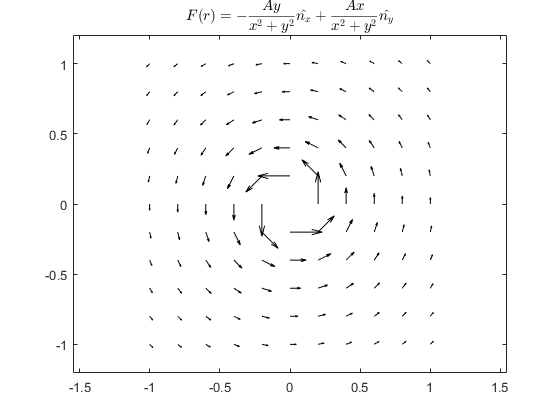
\includegraphics[width=7cm]{p2_a.png}
		\caption{$F(r)=-\frac{Ay}{x^2+y^2}\hat{n_x}+\frac{Ax}{x^2+y^2}\hat{n_y}$}
		\label{fig-2-a}
	\end{figure}
	\begin{align*}
	rot\bar{F}&=\curl\\
	&=\left[\frac{A(x^2+y^2)-2Ax^2)}{(x^2+y^2)^2}+\frac{A(x^2+y^2)-2Ay^2}{(x^2+y^2)^2}\right]\hat{n_z}\\
	&=0
	\end{align*}
	when $x^2+y^2\neq0$
	So the field has zero curl at every point of space except the $z$ axis.
	\item
	Let $x=\cos\theta$, $y=\sin\theta$
	$$F=-A\sin\theta\hat{n_x}+A\cos\theta\hat{n_y}=A\hat{n_{\varphi}}$$
	where $\varphi=\theta+\frac{\pi}{2}$
	$$W=\int_0^{2\pi}A\hat{n_{\varphi}}d\varphi\hat{n_{\varphi}}=2\pi A$$
	\item
	No, although the result of (b) suggests that the force field is conservative while the result of (c) shows that the field did work when a particle moved a circle in it, they do not contradicts with each other. It is because the field is not continuous on the $z$ axis, so that the curl can no longer judge whether the field is conservative. From the result of (c) we can know that the field is not conservative.
	
\end{enumerate}

\section{}
	Suppose the corresponding potential energy at point $(0,0)$ to be zero.
\begin{enumerate}[(a)]
	\item
	$$F(r)=-\frac{\partial U}{\partial x}\hat{n_x}-\frac{\partial U}{\partial y}\hat{n_y}=-(y^2+2xy)\hat{n_x}-(x^2+2xy)\hat{n_y}$$
	\item
	\item
	\begin{figure}[h!]
		\centering
		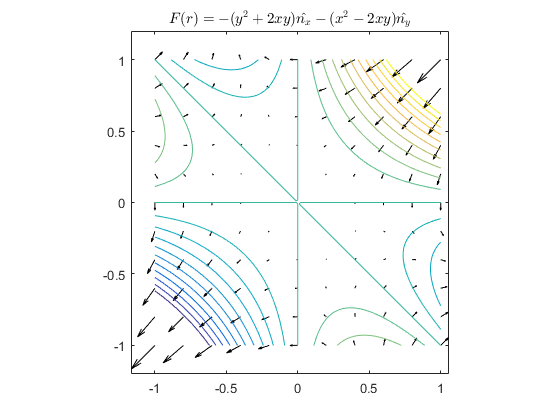
\includegraphics[width=7cm]{p3_a.png}
		\caption{$F(r)=-(y^2+2xy)\hat{n_x}-(x^2-2xy)\hat{n_y}$}
		\label{fig-2-a}
	\end{figure}
	The figure is symmetrical to the line $y=x$\\
	The nearer to the origin, the sparser the equipotential lines.
\end{enumerate}

\section{}
	Suppose right to be the positive direction.
\begin{enumerate}[(a)]
	\item
	Suppose the maximum speed occurs when the block is $x$ cm right of the origin equilibrium point.
	$$\Delta E_p=\frac{1}{2}k_2(x_0^2-x^2)+\frac{1}{2}k_1(x_0^2-x^2)$$
	When $x=0$,
	$$\Delta E_{pmax}=\frac{1}{2}(k_2+k_1)x_0^2=50.625J$$
	$$\Delta E_{pmax}+\Delta E_{kmax}=0\Longrightarrow\frac{1}{2}mv_{max}^2=50.625$$
	$$v_{max}=\frac{3\sqrt{15}}{2}m/s$$
	The max speed occurs at the origin equilibrium point.
	\item
	$$E_{p0}=\frac{1}{2}(k_2-k_1)x_0^2$$
	$$E_{p}=\frac{1}{2}(k_2-k_1)x^2$$
	$$E_{p0}=E_p\Longrightarrow x=-15cm$$
	$$F_m=k_1|x|=375N$$

\end{enumerate}

\section{}
\begin{enumerate}[(a)]
	\item
	$$E_p=mg\Delta h=\rho Shg\Delta h=1000\cdot3.0\times10^6\cdot1\cdot9.8\cdot149.5=4.3953\times10^{12}J$$
	\item
	$$W=0.9\Delta E_p=0.9mg\Delta h=0.9\rho Shg(H-\frac{h}{2})=3.6\times10^9J$$
	$$-\frac{1}{2}h^2+150h-\frac{20}{147}=0$$
	$$h=9.070\time10^{-4}m$$
	$$V=Sh=2721.1m^2$$
	\item
	$$E_p=mg\Delta h\rho Shg\Delta  h=1000\cdot3.0\times10^6\cdot150\cdot9.8\cdot7.5=3.3075\times10^{14}J=9.1875\times10^{7}kWh$$
\end{enumerate}

\section{}
\begin{enumerate}[(a)]
	\item
	$$F(r)=-\frac{dU}{dr}=U_0\left[\frac{12}{r}\left(\frac{R_0}{r}\right)^{12}-\frac{12}{r}\left(\frac{R_0}{r}\right)^{6}\right]$$
	The first term is responsible for repulsion and the second term is responsible for attraction.
	\item
	\begin{figure}[b!]
		\centering
		\subfigure[$U(r)$]{
		\label{Fig.sub.1}
		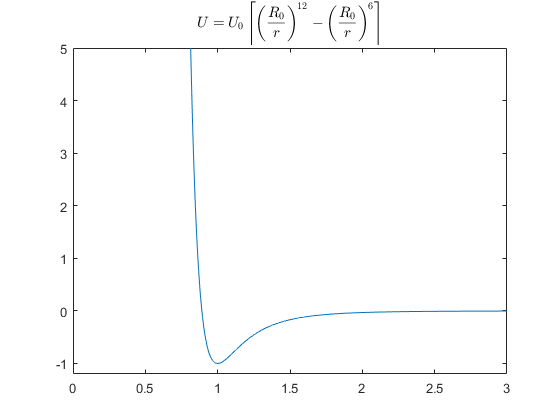
\includegraphics[width=7cm]{p6_a.png}}
		\subfigure[$F(r)$]{
		\label{Fig.sub.2}
		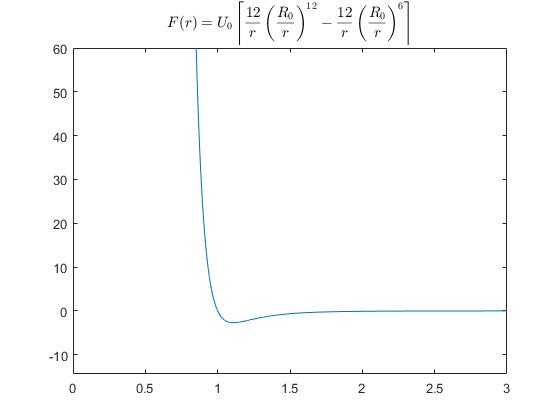
\includegraphics[width=7cm]{p6_b.png}}
		\caption{graphs of both the potential energy and the force}
		\label{fig-sample}
	\end{figure}
	$U_0$ interprets the minimum potential energy associated with interaction between a pair of neutral atoms or molecules.
	
	$R_0$ interprets the distance r between a pair of neutral atoms or molecules at the minimum potential energy associated with interaction between them.
	\item
	$$F(x)\approx-U''(x_0)(x-x_0)=-U_0\left[\frac{156}{R_0^2}\left(\frac{R_0}{R_0}\right)^{12}-\frac{84}{R_0^2}\left(\frac{R_0}{R_0}\right)^{6}\right](x-R_0)=-\frac{72U_0}{R_0^2}(x-R_0)$$
	$$\omega_0=\sqrt{\frac{k}{m}}=\sqrt{\frac{72U_0}{mR_0^2}}$$
	$$T=\frac{2\pi}{\omega_0}=2\pi\sqrt{\frac{mR_0^2}{72U_0}}$$
	$$x(t)=R_0+A\cos(\sqrt{\frac{72U_0}{mR_0^2}}t+\varphi)$$
	\item
	The oscillation near the point $x=R_0$ is a harmonic oscillation.
\end{enumerate}

\section{}
	$$\Delta E_k+\Delta E_p=0\Longrightarrow\frac{1}{2}mv^2=E-U(x)$$
	$$v=\sqrt{\frac{2[E-U(x)]}{m}}=\frac{dx}{dt}$$
	$$dt=\sqrt{\frac{m}{2[E-U(x)]}}dx$$
	Do integrals on both sides,
	$$t=\int_{x_1}^{x_2}\sqrt{\frac{m}{2[E-U(x)]}}dx$$
	$$T=2t=2\int_{x_1}^{x_2}\sqrt{\frac{m}{2[E-U(x)]}}dx$$
\section{}
\begin{enumerate}[(a)]
	\item
	\begin{align*}
	T&=2\int_{x_1}^{x_2}\sqrt{\frac{m}{2(E-U_0\tan^2\alpha x)}}dx\\
	&=\sqrt{2m}\int_{x_1}^{x_2}\cos\alpha x\sqrt{\frac{1}{E\cos^2\alpha x-U_0\sin^2\alpha x}}dx\\
	&=\sqrt{2m}\frac{1}{\alpha}\int_{\sin\alpha x_1}^{\sin\alpha x_2}\sqrt{\frac{1}{E-(E+U_0)u^2}}du\quad(u=\sin\alpha x)\\
	&=\frac{1}{\alpha}\sqrt{\frac{2m}{E+U_0}}\int_{\sin\alpha x_1}^{\sin\alpha x_2}\sqrt{\frac{1}{\frac{E}{E+U_0}-u^2}}du\\
	&=\frac{1}{\alpha}\sqrt{\frac{2m}{E+U_0}}\left[\arcsin\frac{u}{\sqrt{\frac{E}{E+U_0}}}\right]_{\sin\alpha x_1}^{\sin\alpha x_2}\\
	&=\frac{1}{\alpha}\sqrt{\frac{2m}{E+U_0}}\left(\arcsin\sqrt{\frac{E+U_0}{E}}\sin\alpha x_2-\arcsin\sqrt{\frac{E+U_0}{E}}\sin\alpha x_1\right)
	\end{align*}
	\item
	$$F(x)=-U'(x)=-2U_0\tan\alpha x\frac{1}{\cos^2\alpha x}\alpha=-2U_0\alpha\frac{\sin\alpha x}{\cos^3\alpha x}$$
	When $F(x)=0$, $x_0=0$
	$$U''(x_0)=2U_0\alpha\frac{\alpha\cos^4\alpha x_0+\sin\alpha x_0(3\alpha\cos^2\alpha x_0\sin\alpha x_0)}{\cos^6\alpha x_0}=2U_0\alpha^2\frac{\cos^2\alpha x_0+3\sin^2\alpha x_0}{\cos^4\alpha x_0}=2U_0\alpha^2$$
	$$F(x)\approx-U''(x_0)(x-x_0)=-2U_0\alpha^2x$$
	$$T'=2\pi\sqrt{\frac{m}{k}}=\frac{\pi}{\alpha}\sqrt{\frac{2m}{U_0}}$$
	When $E\rightarrow U_0\tan^2\alpha x$,
	$$\arcsin\sqrt{\frac{E+U_0}{E}}\sin\alpha x\rightarrow\arcsin\sqrt{\frac{1+tan^2\alpha x}{tan^2\alpha x}}\sin\alpha x=\arcsin\frac{\sin\alpha x}{|\sin\alpha x|}$$
	When $x_2\rightarrow0^+$, 
	$$\arcsin\frac{\sin\alpha x}{|\sin\alpha x|}\rightarrow\frac{\pi}{2}$$
	When $x_1\rightarrow0^-$, 
	$$\arcsin\frac{\sin\alpha x}{|\sin\alpha x|}\rightarrow-\frac{\pi}{2}$$
	$$T=\frac{1}{\alpha}\sqrt{\frac{2m}{E+U_0}}\left(\frac{\pi}{2}+\frac{\pi}{2}\right)\rightarrow\frac{\pi}{\alpha}\sqrt{\frac{2m}{U_0(1+\tan^2\alpha x)}}=\frac{\pi}{\alpha}\sqrt{\frac{2m}{U_0}}$$
	So we can concluded that in small oscillations, the approx of T is accurate.
	\item
\end{enumerate}
	\begin{figure}[h!]
		\centering
		\subfigure[$U_0=1,\alpha=1$]{
		\label{Fig.sub.1}
		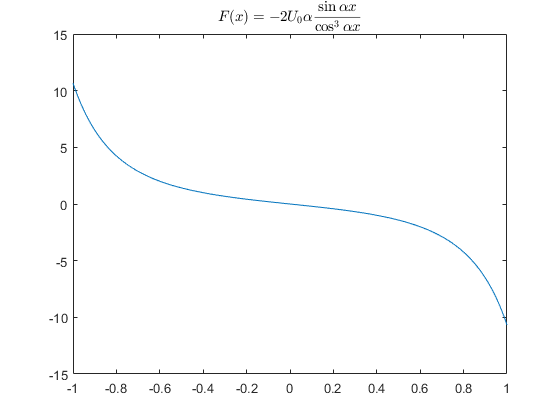
\includegraphics[width=7cm]{p8_a.png}}
		\subfigure[$U_0=0.5,\alpha=0.5$]{
		\label{Fig.sub.2}
		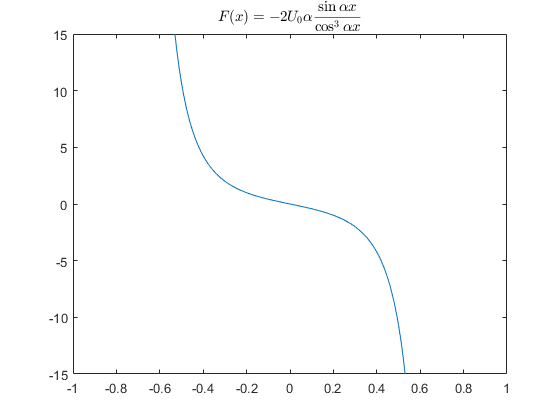
\includegraphics[width=7cm]{p8_b.png}}
		\caption{$F(x)=-2U_0\alpha\frac{\sin\alpha x}{\cos^3\alpha x}$}
		\label{fig-sample}
	\end{figure}
\end{document}
